%% Version 6.1, 1 September 2021
%
%%%%%%%%%%%%%%%%%%%%%%%%%%%%%%%%%%%%%%%%%%%%%%%%%%%%%%%%%%%%%%%%%%%%%%
% amspaperV6.tex --  LaTeX-based instructional template paper for submissions to the 
% American Meteorological Society
%
%%%%%%%%%%%%%%%%%%%%%%%%%%%%%%%%%%%%%%%%%%%%%%%%%%%%%%%%%%%%%%%%%%%%%
% PREAMBLE
%%%%%%%%%%%%%%%%%%%%%%%%%%%%%%%%%%%%%%%%%%%%%%%%%%%%%%%%%%%%%%%%%%%%%

%% Start with one of the following:
% 1.5-SPACED VERSION FOR SUBMISSION TO THE AMS
\documentclass{ametsocV6.1}
\usepackage{makecell}
\usepackage{subcaption}
\usepackage{multirow}
% TWO-COLUMN JOURNAL PAGE LAYOUT---FOR AUTHOR USE ONLY
% \documentclass[twocol]{ametsocV6.1}

%%%%%%%%%%%%%%%%%%%%%%%%%%%%%%%%

%%% To be entered by author:

%% May use \\ to break lines in title:

\title{Lives Saved vs Time Lost: Direct Societal Benefits of Probabilistic Tornado Warnings}

%% Enter authors' names and affiliations as you see in the examples below.
%
%% Use \correspondingauthor{} and \thanks{} (\thanks command to be used for affiliations footnotes, 
%% such as current affiliation, additional affiliation, deceased, co-first authors, etc.)
%% immediately following the appropriate author.
%
%% Note that the \correspondingauthor{} command is NECESSARY.
%% The \thanks{} commands are OPTIONAL.
%
%% Enter affiliations within the \affiliation{} field. Use \aff{#} to indicate the affiliation letter at both the
%% affiliation and at each author's name. Use \\ to insert line breaks to place each affiliation on its own line.

\authors{Alexander Ugarov\thanks{Current Affiliation: HiveReview. The author appreciates support and comments from CIMMS researchers, but most of all Kimberley Klockow and Harold Brooks.},\aff{a}\correspondingauthor{Alexander Ugarov, alugarov@gmail.com} 
}

\affiliation{\aff{a}{University of Oklahoma, CIMMS}}

%%%%%%%%%%%%%%%%%%%%%%%%%%%%%%%%%%%%%%%%%%%%%%%%%%%%%%%%%%%%%%%%%%%%%
% ABSTRACT
%
% Enter your abstract here
% Abstracts should not exceed 250 words in length!
%

\abstract{National Weather Service is planning to implement the system of probabilistic tornado warnings. In this paper, we estimate and compare full societal costs of tornadoes with existing deterministic and potential probabilistic  warnings. These full costs include the value of statistical lives lost as well as the value of the time spent sheltering. We find that probabilistic tornado warnings would decrease total expected fatalities. The improvement in decision-making would also decrease the total oppportunity cost of time spent sheltering even though the total sheltering time is likely to increase. In total, probabilistic warnings should lower societal costs of tornadoes relative to deterministic warnings by approximately 75-150 million USD per year with a large portion of this improvement coming from lower casualties.} 

\begin{document}


%% Necessary!
\maketitle

%%%%%%%%%%%%%%%%%%%%%%%%%%%%%%%%%%%%%%%%%%%%%%%%%%%%%%%%%%%%%%%%%%%%%
% SIGNIFICANCE STATEMENT/CAPSULE SUMMARY
%%%%%%%%%%%%%%%%%%%%%%%%%%%%%%%%%%%%%%%%%%%%%%%%%%%%%%%%%%%%%%%%%%%%%
%
% If you are including an optional significance statement for a journal article or a required capsule summary for BAMS 
% (see www.ametsoc.org/ams/index.cfm/publications/authors/journal-and-bams-authors/formatting-and-manuscript-components for details), 
% please apply the necessary command as shown below:
%
% Significance Statement (all journals except BAMS)
%
\statement
	We measure societal benefits of probabilistic and deterministic tornado warnings in the US by evaluating their effects on expected casualties and sheltering costs. We find that probabilistic warnings deliver almost twice as much net societal benefits as deterministic ones. These gains happen due to less casualties and due to making protective behavior more responsive to risks and sheltering costs.  This paper provides additional evidence of the need to implement probabilistic extreme weather warnings.
%
%% Capsule (BAMS only)
%%
%\capsule
%       Enter BAMS capsule here, no more than 30 words. See \url{www.ametsoc.org/index.cfm/ams/publications/author-information/formatting-and-manuscript-components/#capsule} for details.
% 
%% * * If using twocol mode, you will need to use the commands "twocolsig" and "twocolcapsule" in place of "sig" and "capsule"
%%      to ensure that the text box correctly spans across both columns.


%%%%%%%%%%%%%%%%%%%%%%%%%%%%%%%%%%%%%%%%%%%%%%%%%%%%%%%%%%%%%%%%%%%%%
% MAIN BODY OF PAPER
%%%%%%%%%%%%%%%%%%%%%%%%%%%%%%%%%%%%%%%%%%%%%%%%%%%%%%%%%%%%%%%%%%%%%
%
\section{Introduction}

Most people are aware about grim costs of tornados killing dozens of people per year\footnote{National Weather Service, https://www.weather.gov/media/pah/Skywarn/TORNADOsafety.pdf}, but less know about warnings killing hundreds thousand of hours of sheltering time.  Sheltering is costly because it forces people to reduce time spent on work and leisure. These losses can be plausibly measured in monetary terms: \citet{simmons_economic_2013} estimate that tornados impose roughly 3 to 4 billion USD of annual implicit costs on the US society, and the opportunity costs of sheltering is one of its largest cost components amounting to 1.3-2.6 billion USD.

One proposed way to reduce societal costs of tornados is to provide information on the probability of a tornado to happen in a location instead of providing deterministic yes/no prediction \citep{rothfusz_facets_2018}. In theory, probabilistic extreme weather warnings give more detailed information to users and enable them to make better decisions \citep{murphy_what_1993, papastavrou_improving_1996}.  Potential users in the US also demonstrate preference for receiving probabilistic versus deterministic weather forecasts \citep*{morss_communicating_2008, morss_examining_2010}. At the same time, probabilistic warnings might reduce the decisions quality for some users, and hence it is not clear apriori whether their potential societal benefits would outweigh the additional cost of development and delivery of more sophisticated forecasts.

This paper uses population responses to calculate societal benefits of deterministic and probabilistic tornado warnings. Our calculation of societal benefits accounts for their effects on fatalities, injuries and on sheltering time. We assign monetary measures to fatalities and injuries by using the value of statistical life approach and price the inconveniences of sheltering time based on the concept of opportunity costs of time.

This work involves three steps. First, we conduct a household survey to learn the population's protective responses both to current deterministic tornado warnings and to prospective probabilistic ones. These responses account both for probability levels and for housing types. However, extreme weather alerts do not help if protective responses are inefficient. So, on the second step, we evaluate the efficiency of protective responses conditional on housing type by using the data on historic variation in weather information quality and tornado casualties. Finally, we use the current joint distribution of deterministic forecasts and tornado events to estimate the frequency of probabilistic alerts for each probability level. This last step is important, because it allows us to change the forecasting format while keeping the quality of forecasting technology constant.

The survey collects the data on hypotherical protective responses from the population mostly living in tornado-prone areas. To achieve better representation of diverse populations, it recruits respondents both through mail invitations sent to random addresses in the US Postal Service database and through the Qualtrics Internet-panel. The mail sample includes 718 households with the majority (514) coming from the twenty states with the highest incidence of significant tornadoes. The Internet sample includes 403 responses with 247 responses from English speakers and 156 responses from Spanish speakers with limited English. All the Internet survey responses come from the residents of 20 states with the highest rate of significant tornadoes which are located mostly in Midwest and South of the continental U.S. 

We calculate that probabilistic tornado warnings should create net annual benefits between 78 to 138 million USD depending on the calculation method used. The lower estimate assumes that the population has identical opportunity costs of time, while the larger estimate assumes that these costs vary across individuals. Varying opportunity costs imply that individuals sheltering always do it becayse of facing lower costs of sheltering relative to costs of life or injury. The benefit of probabilistic warnings is relative to deterministic ones, which on their own already create 100-145 million USD per year of net societal value.  This is a rather conservative estimate, because it accounts for imperfect awareness and compliance with warnings and for imperfect protection technology.

Most respondents demonstrate good understanding of probabilistic warnings and good calibration of responses to threat levels. Reported protective responses tend to increase with tornado probabilities. More interestingly, opportunity costs of time implied by their protective responses are consistent with previous estimates of opportunity costs of time in the literature. It supports the idea that potential users correctly deduce their personal risk levels from probabilistic warnings. 

In response to probabilistic alerts, more people report willing to monitor the threat as compared to deterministic warnings, but expect to shelter when the danger becomes imminent.  Many individuals expect to respond to probabilistic warnings even when the tornado probability in a 10-mile radius circle is as low as 10-15\% which we estimate to be below the average implied probability for a deterministic tornado warning. It leads to more people reacting to probabilistic warnings and eventually more people taking selter. As a result, probabilistic warnings reduce total casualties. At the same time, probabilistic warnings increase the total time spent sheltering or monitoring the weather. This increase does not necessarily converts to higher societal costs. If we account for optimal response to predicted tornado probabilities and deduce opportunity costs from reported protective responses, then the societal value or opportunity cost of sheltering/monitoring time goes down due to more graduated reaction to probabilistic warnings. Probabilistic warnings deliver this positive effect by enabling users with higher opportunity costs to shelter only if tornado threats are sufficiently high. 

We contribute to the literature by directly measuring net benefits of both deterministic and probabilistic tornado warnings. Similar to our study, \cite{howard_firm_2021} measure economic benefits of probabilistic warnings for businesses and find that they allow firms to save extra 1.3-5.6 billion USD per year. With respect to  general population, \citet{simmons_economic_2013} calculate that contemporary societal costs of tornados are roughly 6 billion USD lower than the hypothetical costs with tornado lethality at the 1925 US level and with no warnings. However, this change cannot be completely attributed to the effect of deterministic tornado warnings, because other safety improvements happen simultaneously during this period. This paper takes a more conservative approach to estimate the benefits of both deterministic and probabilistic warnings by accounting for imperfect compliance with warnings and by calculating their efficiency directly from the variation in casualties between warned and non-warned populations. 

In contrast to our approach, multiple other studies of economic value of weather information \citep{lazo_economic_2002, lazo_300_2009, lazo_valuing_2011, wehde_public_2021-1} use the contingent valuation method in which potential users directly report their willingness-to-pay for the service. Most relevant for our study, \citet{wehde_public_2021-1} find that the US population is willing to pay on average \$7.5 per person for an app providing probabilistic graphical tornado alerts. This price translates to one-time aggregate benefit between 900 million to 1.56 billion USD depending on aggregation assumptions used. While contingent valuation studies can potentially reflect additional benefits of information such as peace of mind or increased safety of others, they suffer from the hypothetical bias emerging due to respondents deliberately overstating their willingness-to-pay \citep{blumenschein_eliciting_2008, johnston_contemporary_2017}.  As a result, contingent valuation studies often provide excessively high and varying estimates of economic benefits. Hence a direct approach we use provides an important and more reliable lower bound of the new system's value. 

Our study supports the conclusion that the US population can interpret and use probabilistic warnings. Multiple previous studies \citep{ash_tornado_2014, lindell_perceptions_2016, miran_user_2017-1} test perception and hypothetical responses to graphical representation of probabilistic severe weather alerts. In general, they find that people increase protection in response to increasing threat probabilities, even though presentation formats have strong influence both on average response levels and on sensitivitiy of response to presented probabilities. Additionally, \cite{leclerc_cry_2015} find that probabilistic information improves decision-making and reduces the "cry-wolf" effect, while \citet{krocak_exploring_2022} find that probabilistic information allows for better decision-making compared to categorical verbal descriptions of uncertainty. We do not only find that protective responses are sensitive to projected probabilities, but also that response levels are well-calibrated to threat levels and consistent with choices made in other domains (such as speeding \citep{wolff_value_2014}).



\vspace{20pt}

\section{Survey Design and Implementation}

\vspace{10pt}
\subsection{Data Collection} 
We collect the data from two samples. The mail survey recruited respondents across the whole US but with the emphasis on tornado-prone regions (see Table \ref{tor_prone} in the Appendix). Respondents could choose to respond by mail by using an enclosed envelope or to fill the survey online. The Internet-survey recruited subjects from the tornado-prone regions only. The use of different sampling methods intended to get a wider representation of different demographic groups. Mail survey reached more older respondents living in rural communities, while the Internet-survey helped to get answers from younger respondents. We received 718 responses from the mail survey and 403 responses from the Internet survey. Questionnaires were practically identical  except for small changes needed to screen respondents in the Internet survey. 

% latex table generated in R 4.0.2 by xtable 1.8-4 package
% Wed Dec 16 14:45:07 2020
\begin{table}[htbp!]
 \caption{Internet Survey Sample}
\label{descr_q}
\footnotesize
\centering
\begin{tabular}{lcccccc}
\hline
\hline
 & \multicolumn{3}{c}{\textbf{Good English}}& \multicolumn{3}{c}{\textbf{\makecell{Lim. English \\Hispanics}}} \\
\hline
 & \multicolumn{2}{c}{Sample}& Popul. &\multicolumn{2}{c}{Sample} & Popul.\\
 & N & \% & \% & N &  \% &  \% \\ 
  \hline
Male & 97 & 39 & 49 & 48 & 31 & 47 \\ 
  $<$35 & 52 & 21 & 30 & 55 & 35 & 21 \\ 
  35-59 & 97 & 39 & 41 & 87 & 56 & 54 \\ 
  60+ & 98 & 40 & 29 & 14 & 9 & 25 \\ 
  No school & 0 & 0 & 1 & 6 & 4 & 9 \\ 
  Grades 1-12, no HS diploma & 11 & 4 & 8 & 21 & 13 & 46 \\ 
  HS diploma & 54 & 22 & 34 & 48 & 31 & 29 \\ 
  Some college & 56 & 23 & 26 & 21 & 13 & 7 \\ 
  Associate or bachelor's degree & 76 & 31 & 20 & 50 & 32 & 6 \\ 
  Advanced degree & 50 & 20 & 11 & 10 & 6 & 2 \\ 
  White & 197 & 80 & 77 & 88 & 56 & 74 \\ 
  Black & 28 & 11 & 16 & 6 & 4 & 1 \\ 
  Asian & 6 & 2 & 3 & 1 & 1 & 0 \\ 
  Native American & 2 & 1 & 1 & 2 & 1 & 1 \\ 
  Other & 6 & 2 & 2 & 56 & 36 & 23 \\ 
  Mixed & 8 & 3 & 2 & 3 & 2 & 1 \\ 
   \hline
\end{tabular}
\end{table}
\label{sample_tab}

The mail survey uses stratified probabilistic sampling to get a more representative sample which allows us to use statistical tests. Our initial frame comes from the USPS delivery route database. We stratify the sampling frame by state of residence and by housing type and sample 10600 addresses with more addresses from tornado-prone states. We consider the state to be tornado-prone if it belongs to 20 states with the highest average incidence of significant tornadoes (EF2 and above) per square mile within the last 20 years.  The selected states include 45\% of the US population, but 88\% of tornado fatalities. This paper uses only the sample obtained from the tornado-prone states.

The questionnaire was pretested, first, by using qualitative personal  interviews conducted either in person or over Google Meets and Skype. These interviews helped us to clarify the question's wording and make sure that their interpretation by subjects matches our expectations. On the second stage, we conducted quantitative pilots both for the Internet-sample and for the mail survey.

We pretest our surveys by using, first, qualitative face-to-face\footnote{Due to COVID-19 pandemic, we conducted most of the qualitative interviews online either through Zoom, Skype or Google Meets.} interviews and, second, through quantitative pilot studies. The qualitative interviews help to clarify the understanding of questions and refine the lists of response options. The interview followed think-aloud protocols \citep{dillman_internet_2008} in which respondents  read all the questions aloud and vocalize their thinking process. Quantitative pilots followed the same procedure we intended to use for the main study but with smaller samples. We conducted two pilots for the Internet-sample and two pilots (400 and then 200 letters) for the mail survey. Our pilots helped to adjust our sampling strategies and redesign a few questions which turned to be ambiguous to the subjects.

\vspace{10pt}
\subsection{Representativeness and Selection Bias} 
Despite our effort to use different recruiting efforts, both samples had disproportionally more females and more people with college education and above (Table \ref{sample_tab}). Additionally, the mail survey recruited more older white respondents. Hence in order to translate our findings to the US population we re-weight our results to match the US population structure by age and gender.\footnote{We use the datafrom the American Community Survey 2018, downloaded from IPUMS (\citet{ruggles_ipums_2021}).}



\vspace{20pt}
\section{Use of Standard and Extended Tornado Alerts}

First, we study how extended tornado warnings would affect protective responses. We ask our respondents to imagine being at home with their family at 7 PM when a tornado warning is issued. Next, we elicit their protective responses conditional on lead times and on probabilities of a tornado to happen within a given time interval. The Internet-survey asks the same set of questions for the nightime warnings (2 AM).\footnote{Mail survey conducted after the Internet-survey had to drop these questions in effort to shorten the questionnaire.} While these questions cannot describe the multitude of scenarios for different times and for different circumstances (such as staying outside or being separated from the family), we still believe that they cover the most common scenario. 
\begin{figure}[!htbp] 
\centering
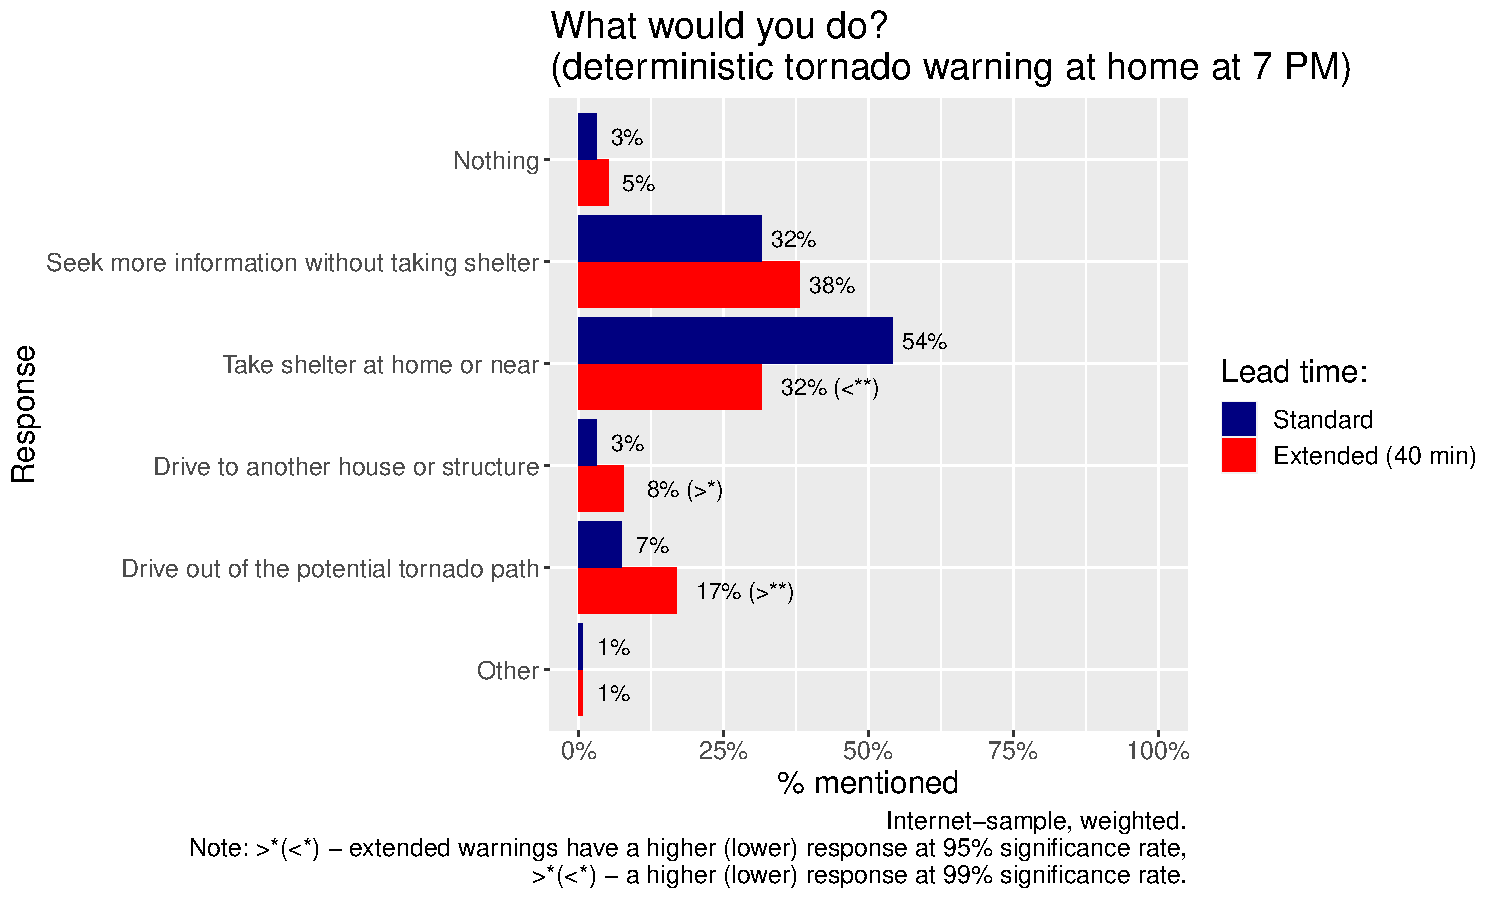
\includegraphics[width=33pc]{../Graphs/contr_plot_allQ.pdf}
\caption{Protective Response by Lead Time (Internet-sample)}\label{contr_plot}
\end{figure}
Most respondents choose to respond to a standard tornado warning by taking a shelter at home or near.  The proportion of respondents choosing this action (55\%) is surprisingly stable across samples and across times in the same sample (Figure \ref{contr_plot}). Roughly one-third of responds expects to seek more information without taking shelter. About 10\% of respondents in the Internet sample choose to drive to another house or structure or to drive out of the potential tornado path. This proportion is even lower for the mail sample (Figure \ref{comp_responses}).

Increasing lead time to 40 minutes on its own have practically no effect on the total proportion of people taking any protective action, as more than 90\% of individuals do it anyway. However, increasing lead time decreases the likelihood of sheltering at home in favor of seeking more information and evacuating. It is clear that extended lead time improves safety of people in vulnerable housing conditions, such as mobile houses. But the safety of people living in more robust homes depends on their ability to interpret additional information they receive while not sheltering and properly responding to it.

Providing probabilistic information is the most crucial aspect of prospective tornado alerts system, but their usefulness relies on the users' ability to understand and react to probabilistic forecasts. The survey indicates that most individuals respond rationally to probabilistic warnings. The proportion of respondents choosing to protect increases with the forecasted probability. Almost 100\% of respondents expect to take some protective action if they learn that a tornado would happen with probability 100\% in the next 40 minutes in a 10 mile radius from their location. Less than 5\% of respondents make non-monotonic choices meaning that 95\% of respondents protect for all the probabilities which are higher than their threshold probability.
\begin{figure}[!htbp]
\centering
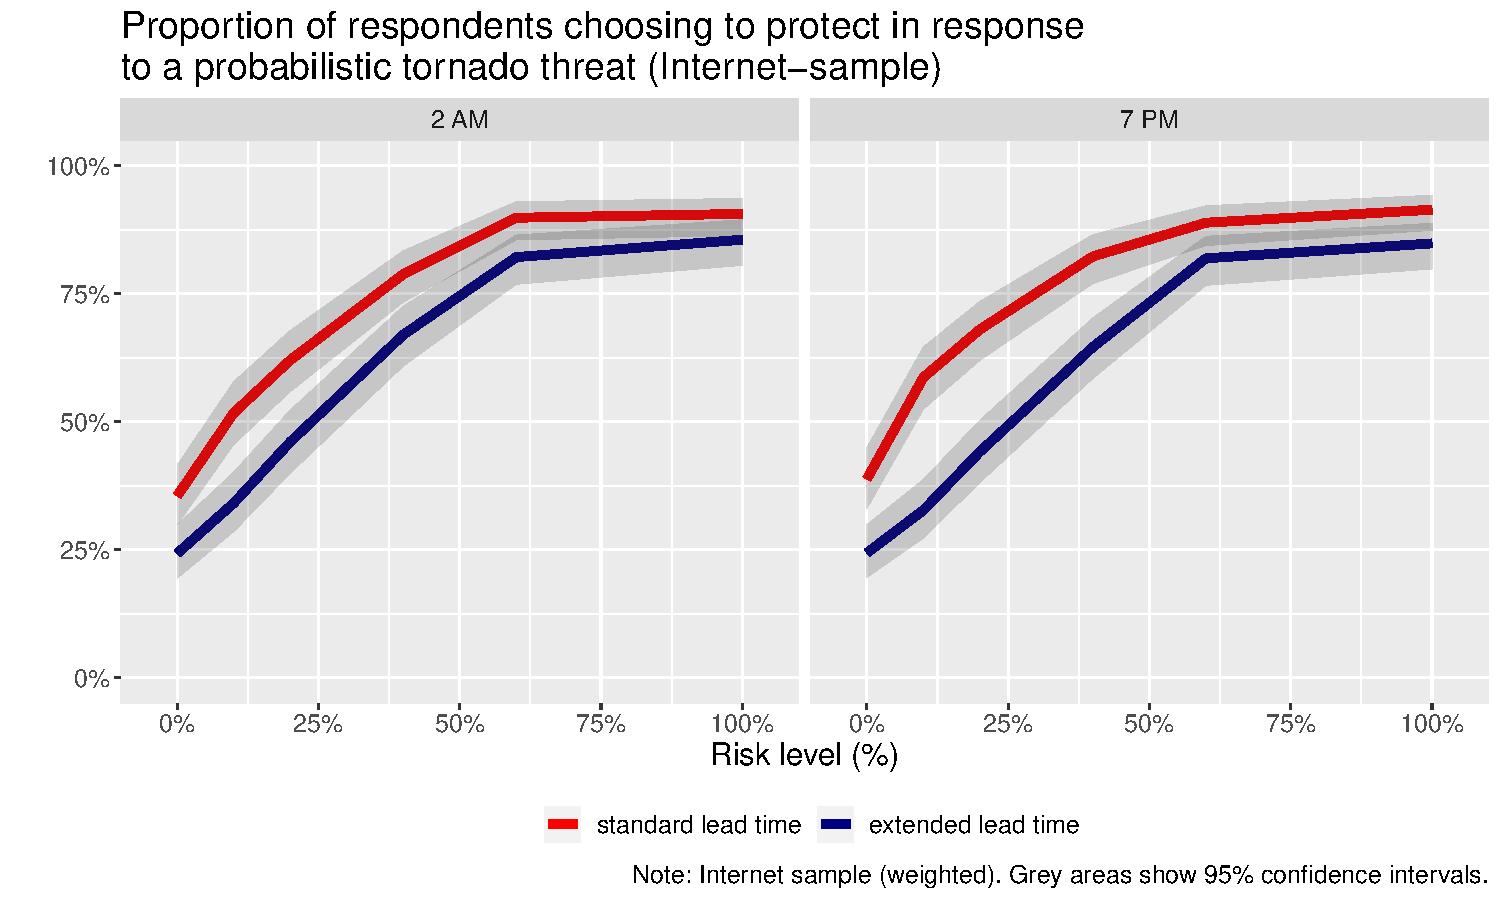
\includegraphics[width=33pc]{../Graphs/threat_resp_allQ.pdf} 
\caption{Protective Response by Probability of a Tornado (Internet sample)}\label{threat_respQ}
\end{figure}
Our analysis presented in Figure \ref{threat_respQ} shows that most individuals expect to first take protective actions when the probability gets to 40\%.\footnote{This is easy to see through the slope of the curves in Figure \ref{threat_respQ}.} Interestingly, this is the probability most consistent with implied probabilities of existing deterministic tornado warnings, which also prompt the majority of users to protect. The reaction threshold is higher for nighttime warnings. This is consistent with higher costs of nighttime protective actions for most respondents as they potentially require interrupting sleep and driving with poor visibility.




\vspace{20pt}
\section{Computation of Direct Societal Benefits}
\vspace{10pt}
\subsection{Overview of the Approach} 

We estimate direct economic benefits of extended tornado warnings as the difference in direct societal costs between standard and extended warnings. Direct societal costs in our calculation include the cost of tornado deaths and injuries and the cost of time spent sheltering (Sheltering Costs). This approach is similar to the approach used by \citet{simmons_economic_2013}. We convert each of the cost components to the monetary scale. Value of statistical life and value of statistical injury metrics translate predicted numbers of deaths and injuries into equally undesirable monetary costs. We use the Value of Time to price the time spent sheltering under both standard and extended tornado alerts. Direct costs of tornadoes is:
$$\mbox{Direct Costs }=\mbox{ VSL Lost }+\mbox{ Value of Injuries }+\mbox{ Sheltering Costs}$$
Value of statistical life (VSL) assigns a monetary value to life based on observed trade-offs between money and small chances of death. Based on literature review for wage differentials for risky occupations, \citet{viscusi_value_2003} suggest the range from \$7 million to \$12.4 million per statistical life. We use VSL of \$11.13 million which is equal to the value recommended by \citet{kniesner_value_2019} and adjusted for inflation from 2019 to 2020. For comparison, \citet{simmons_economic_2013} use the value of \$7.6 million per statistical life in prices of 2007, which corresponds to \$9.5 million in 2020 prices.  The US Environmental Protection Agency recently used the value of \$10.9 million in its Emission Guidelines for Greenhouse Gas Emissions from Existing Electric Utility Generating Units (2018)\footnote{https://www.epa.gov/stationary-sources-air-pollution/electric-utility-generating-units-emission-guidelines-greenhouse}, which also translates to \$11.2 million in 2020 prices.

We  assign monetary value to injuries in a similar fashion. Most tornado injuries are minor, and so following the approach in \citep*{simmons_direct_2006, simmons_economic_2013}, the monetary value of injury is 1/100 of the value of statistical life which is \$86,000 per injury.

The following formula calculates expected injuries and fatalities\footnote{To save on notation, we use the same variable names to denote both expected injuries and expected fatalities. The formulas are identical.} under deterministic warnings as the product of the affected population ($P_A$), baseline injury/fatality rate ($r$) in the affected population and the mitigation factor due to protective responses ($M$):
$$F_D=P_A \times r \times M$$
Affected Population ($P_A$) is the expected annual population in tornado strike zones. It is equal to the product of the average annual number of tornado warnings $N_w$, average tornado strike area $A$ and population density $d$ corrected for the false alarm rate (FAR) and probability of detection (POD):
$$P_A= N_w \times A \times d \times (1-FAR)/POD$$
The US issues $N_w=2063$ warnings per year on average (\citet{howard_firm_2021}). The population density in 20 states with the highest frequency of significant tornadoes is $d=119$ people per square mile. \citet{simmons_economic_2013} estimate that the average tornado strike area $A$ is approximately 0.3 square miles. We also use estimates of $POD=0.7$ and $FAR=0.7$. Based on this calculation, Affected Population $P_A$ includes 31.8 thousand people per year. 

The baseline fatality (injury) rate per person in a strike area $r$ is the probability that a person in a tornado strike zone is killed (injured) in a tornado if they do not protect. The protective mitigation factor $m$ measures the proportional decrease in risk of injury/death from the expected protective response. It depends both on the expected behavior and on the efficiency of this behavior in reducing the risk. These two variables strongly depend on housing conditions, so we condition our calculation on living in permanent vs. mobile houses and weight by corresponding population proportions. We explain the calculation of the baseline fatality and injury rates and the protective response mitigation factors in the next subsection.

We use a similar approach to forecast casualties under probabilistic forecasts, but now we account for different responses for each tornado probability. We also need to make sure that probabilistic forecasts do not under-predict or over-predict tornadoes. For this purpose, the affected population $P_A$ stays constant between different forecasting approaches. As a result, the probability of a tornado to happen enters the casualty calculation only indirectly through the population's protective response. The expected number of casualties for each predicted probability $F(p)$ is the product of the population affected $P_A$, baseline risk $r$ and probability-specific mitigation factor $M(p)$:
$$C(p) = P_A \times r \times M(p)$$
The total expected number of casualties for the probabilistic forecast $F_P$ is the sum of casualties for each predicted probability $C(p_i)$ weighted by frequency of forecasting each probability $f(i)$:
$$F_P=\sum_i f(i)C(p_i)=\sum_i f(i) \times r  \times M(p_i)$$
The survey describes protective responses to both existing deterministic and prospective probabilistic alerts. For the protective response, we assume that people who report needing to collect more information will eventually shelter before a tornado. \citet{hammer_response_2002} and \citet{klockow_investigation_2011} show that most people in a tornado strike zone take shelter, but fewer people do it in a tornado warning zone \citep*{liu_assessment_1996, sherman-morris_tornado_2010}.

\vspace{10pt}
\subsection{Protective Response Efficiency} 
Protective response mitigation factor $M$ measures the proportional effect of protective actions on tornado fatalities and injuries. Because we are not aware of any generalized estimates of protective response efficiency in the literature, we estimate it indirectly from casualty effects of tornado warnings and other historical data. This estimation assumes that households protect only in response to warned tornadoes, and that the protection response is not universal. We also assume that the protective response has the same proportional effect on reducing both fatalities and injuries.

\citet{simmons_false_2009} find that the warned tornadoes on average have 30-40\% less injuries controlling for tornado strength, strike area, geography, and time. Similarly, \citet{simmons_wsr-88d_2005} find that when a Weather Forecast Office (WFO) in the US installs a WSR-88 weather radar, tornado injuries in covered counties go down by approximately 40\%. Based on this evidence, we make a relatively conservative assumption that warnings reduce injuries by 35\%. While the paper does not observe the effect of warnings on fatalities, this is likely the result of a much smaller number of fatalities in the sample. Consistent with these observations, we also assume that warnings reduce fatalities by 35\%.

The following more technical calculation then infers protective response efficiency. The calculation accounts for housing type $t$ (permanent, mobile) to reflect much higher vulnerability of people living in mobile homes. The effect of protective response depends both on the probability of a response and on its efficiency in reducing casualties. Let $r_t^0$ denote the baseline probability of death for an unprotected person in home of type $t$ in a tornado strike zone and $r_t^w$ is the probability of death for a protected person. Additionally,  $R_t$ is the probability of protective response to a warning and $m_t$ is the mitigation efficiency (for example, an action with $m=0.6$ reduces casualties by 40\% relative to the baseline). Then the casualty rates are described by the following expressions for each type of housing $t$ with $P_t$ denoting the corresponding population share:
\begin{equation}
r^w_t=r^0_t(R_tm_t+(1-R_t)),t=mobile,permanent 
\end{equation}
Next, we assume that warnings reduce casualties by 35\%:
\begin{equation}
\sum_t P_t (r^0_t-r^w_t)=0.35 \sum_t P_t r^0_t,t=mobile,permanent 
\end{equation}
Finally, the average fatality rate $r_t^av$ is the weighted average for warned and unwarned fatality rates accounting for the probability of detection (POD):
\begin{equation}
r_t^av=PODr_t^w+(1-POD)r_t^0,t=mobile,permanent     
\end{equation}
Next, we solve the system of equations above to find both baseline hazard rates $r_t$ and mitigation efficiency parameters $m_t$. As a first step, we consider the population living in mobile homes. \citet{simmons_economic_2013} estimate the average probability of death of mobile home resident $r_{mob}^{av}$ to be 0.8472\% if located in a tornado strike zone. The best and practically the only protection response for a mobile house resident is to evacuate to a sturdier building, shelter or travel out of the tornado path \citep{schmidlin_tornado_2009}. We assume for simplicity that evacuation eliminates the tornado risk for this group ($m_{mob}=0$). However, \citet{schmidlin_tornado_2009} find that only around 30\% of mobile house residents currently evacuate if they receive a tornado warning. Using equations (1) and (3), we obtain that the baseline rate of fatalities for mobile house residents is 110\% of the average or 1.01\% and the warned rate is 0.751\%.

Next, we estimate the baseline risk and the mitigation efficiency for residents of permanent homes. We do it by substituting the risks of mobile home residents into the equation (2) and solving the resulting system of (1-3) for $r_{perm}^0$ and $r_{perm}^w$. The estimate for the average risk of fatalities in permanent homes comes again from \citet{simmons_economic_2013}, who calculate that 0.0882\% of residents in permanent homes die in the average tornado strike zone. We calculate that the baseline risk of death for residents of permanent homes $r_{perm}^0$ is 0.126\% and the risk for warned residents of permanent homes $r_{perm}^w$ is 0.0743\%. Thus, warnings reduce fatalities in permanent homes by roughly 40\%. 

To calculate the mitigation efficiency factor $m_{perm}$ for residents of permanent homes, we need to account for imperfect compliance with issued warnings. Previous studies indicate that while the response rate to warnings $R_{perm}$ is close to around 30\% for warned counties (Liu et al, 1996; Schmidlin et al, 2009), the response rate reaches 70-90\% for population directly in a tornado path and for stronger tornadoes \citep*{klockow_investigation_2011, paul_predictors_2015}. As only the response of individuals in a path matters for casualties, we assume that 60\% of permanent homes residents in a tornado path take some protective action ($R_{perm}=0.6$). It follows that taking protective actions mitigates the baseline risk for permanent homes by approximately 65\% ($m_{perm}=0.361$). 

Event studies support our finding of high mitigation efficiency for permanent homes. For example, \citet{niederkrotenthaler_injuries_2013} finds that sheltering in a basement reduced injuries by roughly 80\% during April 2011 Alabama tornadoes, while \citet{daley_risk_2005} find no severe injuries and deaths among people doing it during the Oklahoma-city 1999 tornado. The same applies for the 2011 Joplyn tornado \citep*{paul_predictors_2015}. The evidence for using interior rooms as a shelter is more mixed. \citet{niederkrotenthaler_injuries_2013} find that sheltering in an interior room had reduced the risk of injury by about 60\%, but \citet{daley_risk_2005} find just 20-30\% reduction in severe injuries and \citet{hammer_response_2002} find no effect of using an interior room vs any other room in a permanent house.

We apply the same approach to the calculation of injury risks. The calculation assumes the average risk of injury at 0.025 for mobile homes in the strike area and the risk of 0.0224 for permanent homes in the strike area (based on Simmons and Sutter, 2013 calculation). The baseline risk of injury for permanent homes equals 0.0306 and the baseline risk for mobile homes equals 0.0316. While the predicted injury risk is very similar for both home types, it seems that permanent homes give a better protection against death, but little protection against non-fatal injuries.


\vspace{10pt}
\subsection{Distribution of Probabilistic Forecasts} 
Population's protective responses depend on perceived probabilities. Hence we need to know how often each probability is forecasted in order to estimate the costs of probabilistic warnings. This task is non-trivial, because for any probability of a tornado, one can issue different unbiased probabilistic forecasts. For example, one completely unbiased but also completely useless forecast is the forecast which is always equal to the baseline (environmental) probability of a tornado to happen. On the opposite end of the precision spectrum, forecasters can predict a probability of 1 if a tornado is going to happen and zero otherwise. In practice, dynamic properties of weather systems and imperfect information impose constraints on the maximum precision of tornado forecasts.

We are going to use signal detection theory to infer the distribution of probabilistic forecasts from the joint distribution of tornado warnings and tornado events.\footnote{\citet{howard_firm_2021} use a simpler approach by assuming equal forecasting frequency for each probability. However, this approach can easily over-estimate the precision of probabilistic forecasts and their value, because it implies a mugh higher average confidence of forecaster than allowed by the existing technology.} The signal detection approach assumes that probabilistic forecasts use the same information as existing standard warnings. If it is indeed true, all the information can be aggregated to one signal equal to the posterior probability of a tornado to happen. In the simplest case which we use here, this signal has a normal distribution with dispersion 1\footnote{One can always rescale the signal without the loss of generality to get the dispersion to equal one.} and a mean depending on actual state of the world. If the state of the world is indeed the state in which a tornado forms, the signal has a higher mean. The difference between signal means in tornadic and non-tornadic state $D'$ measures the forecaster's ability to discriminate between two states of the world.

\citet{brooks_tornado-warning_2004} demonstrates how to use the historic performance of tornado warnings to estimate the difference in means $D'$ between the latent signal distribution in tornado and non-tornado states. \citet{brooks_long-term_2018} use the same approach and estimate that in recent years, the performance is consistent with $1<D'<1.4$ if the baseline probability of a tornado conditional on a storm is 10\%. We use $D'=1.35$ on the upper end of this range to reflect improvements in warnings performance in early 2000's and potential improvements due to better satellite data and dual polarization radars in more recent years. 

The projected distribution of probabilistic forecasts then comes from Monte-Carlo analysis. We draw $N=100,000$ binary events $\omega$ from the set $\{0,1\}$ in which 1 is a tornado state emerging with probability $p_0=0.1$ and then draw $N$ random signals from the corresponding normal distributions ($N(0,1),N(D',1)$). Then we calculate the posterior probability $f$ by using the Bayes formula:
 $$f={p_0\phi(S;D')\over (p_0\phi(S;D')+(1-p_0)\phi(S;0))}$$
Here  $\phi(S;x)$ is a normal distribution density with mean $x$ and $\sigma=1$ which is calculated when the signal equals $S$ .The formula would never produce certain forecasts, but it can get very close to certain forecasts if the signal's value $S$ is very high.
 
\begin{figure}[!htbp]
\centering
\begin{subfigure}{0.45\linewidth}
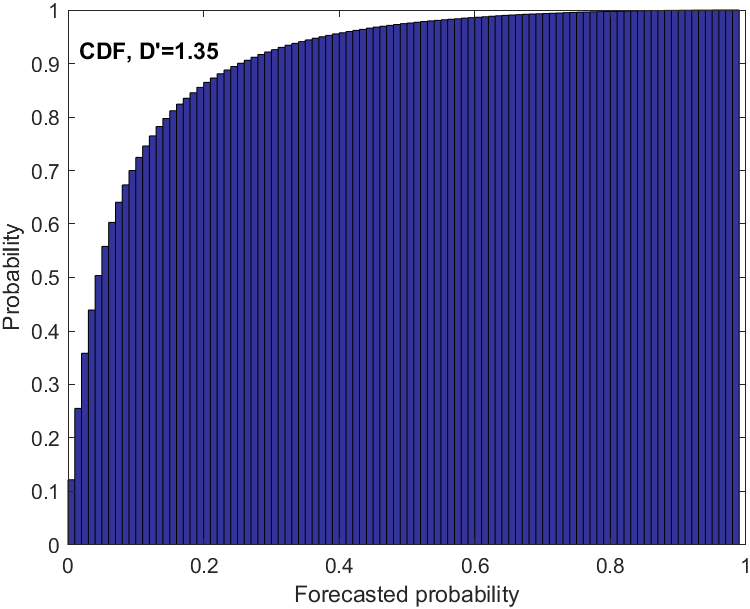
\includegraphics[width=17pc]{../Graphs/cdf_forecast0.png}
\end{subfigure}
~
\begin{subfigure}{0.45\linewidth}
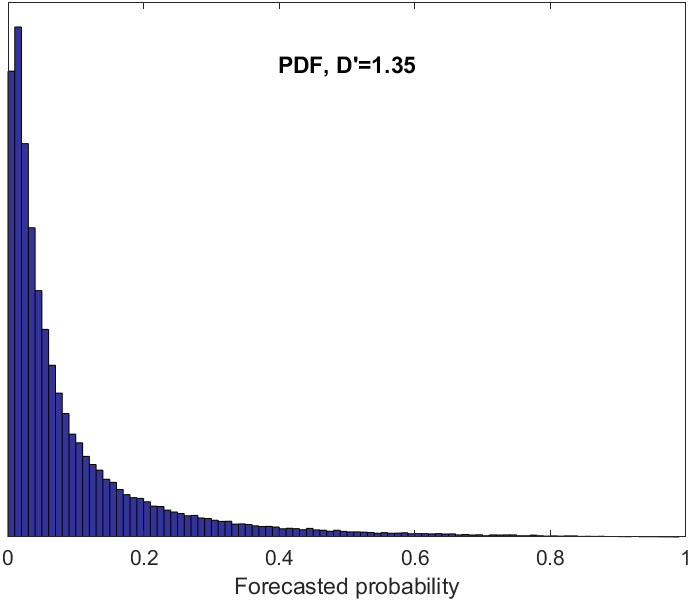
\includegraphics[width=16pc]{../Graphs/pdf_forecast0.png}
\end{subfigure}\caption{Projected Distribution of Probabilistic Tornado Forecasts}\label{prob_forecast}
\end{figure}

The resulting distribution of forecast probabilities (\ref{prob_forecast}) is concentrated around low-probability events, which follows from both low baseline probability of a tornado and our relatively modest ability to forecast tornados.\footnote{It is arguably much harder to forecast a tornado 10 minutes in advance than to forecast rain one hour in advance.} Only 2.5\% of forecasts predict probabilities above 50\%. However, 30\% of forecasts predict that chances are above the baseline 10\% and 14.5\% predict that chances of a tornado are above 20\%.


\vspace{10pt}
\subsection{Sheltering Costs}
Opportunity costs of sheltering reflect the disutility of sheltering instead of continuing normal activities. It is equal to the product of value of time per total annual number of hours  spent sheltering in each scenario. Obviously, value of time depends on activities interrupted and their utility versus the utility of sheltering which can drastically differ both by individual and by time of the day. For example, a person sleeping in their basement do not have to interrupt this activity for sheltering and hence has exactly zero value of time for sheltering. In contrast, a person working at home in an unsafe location might need to stop working which either reduces their earnings roughly by wage rate per hour or reduces their remaining leisure time.  

The total number of hours spent sheltering equals the number of people warned during a typical year $P_w$ multiplied by the average duration of warnings. We use the following formula to calculate the expected annual population warned $P_w$ for deterministic warnings:\footnote{We count one person multiple times if he/she receives multiple warnings during the year.}
$$P_w= N_w \times A_w \times d $$
We again follow \citet{howard_firm_2021} in using the average warning area $A_w=275$ sq. miles and the average number of $N_w=2063$ warnings per year. The population warned for probabilistic warnings is adjusted proportional to the ratio of current probability of event in deterministic forecasts to their average probability of event properly adjusted for area. Our survey describes a positive event as a tornado within 10 miles of the house or closer which corresponds to a slightly larger area (314 sq. miles) than the average area of deterministic impact-based warning, so the adjustment increases the population warned in probabilistic forecasts by a factor of 1.14=314/275 even before adjusting for probabilities.

Because paid work is one of the main activities conducted by working adults, the wage rate provides a natural benchmark for the value of time. However, multiple studies find that even for working adults the value of time is significantly lower than their wage rate. For example, \citet{larson_revealing_2004} find that the value of time varies from 0.5 for adults with fixed week to 0.8 for adults with flexible workweek. \citet{wolff_value_2014} put the value of time as 50\% of the wage rate based on the analysis of speeding tickets and gasoline consumption. Given the large proportion of individuals out of labor force in our sample, we use 1/3 of the average wage rate to value the sheltering time. The average civilian non-farm wage was equal to \$29.35 in 2020. It corresponds to our opportunity cost of sheltering time of \$9.8 per hour.

Most value for probabilistic warnings comes from heterogeneity of their users in terms of costs of sheltering versus safety concerns. Probabilistic warnings allow rational sheltering decisions based on individual cost-benefit analysis with respect to predicted probabilities. For example, a person in a well-protected house might decide against sheltering if the probability is 20\%, but will shelter when the probability increases to 60\%. 

Our alternative calculation of direct costs of tornado warnings accounts for heterogeneous opportunity costs of sheltering. We infer heterogeneous opportunity costs from protective responses reported in the survey similarly to the approach used for firms in \citet{howard_firm_2021}. Subjects report their protective response for each probability of a tornado $p$ which allows us to infer their opportunity costs in the following way. First, for each probability level $p$, not sheltering imposes a certain increase in fatality risk $c(p)$ which we value similarly by using the value of statistical life approach. We calculate the cost of fatality risk $c(p)$ as the product of tornado probability $p$, baseline fatality risk $r$, the efficiency of mitigation measures $(1-m)$, and the value of statistical life $VSL$:
$$c(p)=p \cdot r \cdot (1-m) \cdot VSL$$
Next, we assume that individuals switching from not sheltering to sheltering at probability $p$ do so because their opportunity costs of sheltering start to exceed the fatality costs of not sheltering $c(p)$. In other words, we assume that individuals behave consistently with cost-benefit analysis and successfully evaluate their fatality risks.  If an individual does not shelter in response to the forecast with the probability $p_1$ and associated costs $c(p_1)$, but does so when the probability increases to the level $p_2>p_1$, then the individual's latent opportunity costs of time $c_o$ should be in between these two costs:  $c(p_1)\leq c_o\leq c(p_2)$. This gives a range of plausible opportunity costs for each group of subjects with identical probabilistic thresholds. The upper estimate comes from the assumption that individuals switching when probability increases from $p_1$ to $p_2$ have opportunity costs based on higher probability $p_2$. The lower bound estimate uses the lower probability $p_1$ to calculate sheltering costs and does so for each probability range.  The true value of sheltering costs for each group has to lie somewhere in between higher and lower bounds. Using the largest value of the range of plausible opportunity costs produces more conservative estimates of tornado warnings' value. It also eliminates the need of inferring zero opportunity costs for subjects protecting for the lowest possible probability of 20\%. However, we also show calculation of opportunity costs  under the lower bound approach. We assign the probability $0.0463$ as the risk for the lowest group which corresponds to the average tornado probability conditional on having a storm and on the probabilistic forecast being below 20\%.

% latex table generated in R 4.0.2 by xtable 1.8-4 package
% Fri Nov 25 13:22:03 2022
\begin{table}[!htbp]
\caption{Distribution of Opportunity Costs}\label{opp_costs}
\centering
\begin{tabular}{lccc}
  \hline \hline
Housing & Population share (\%) & \multicolumn{2}{c}{Value of Time (USD per hour)} \\ 
 &  & Lower est. & Upper est. \\ 
  \hline
\multirow[c]{6}{*}{Permanent}  & 58.43 & 0.78 & 3.35 \\ 
 & 21.09 & 3.35 & 6.71 \\ 
 & 11.06 & 6.71 & 10.06 \\ 
  & 3.69 & 10.06 & 13.41 \\ 
 & 0.45 & 10.06 & 16.76 \\ 
 & 5.31 & 16.76 & $>$16.76 \\ 
\hline
\multirow[c]{6}{*}{Mobile} & 17.69 & 8.87 & 38.31 \\ 
 & 9.61 & 38.31 & 76.62 \\ 
 & 9.22 & 76.62 & 114.93 \\ 
& 5.00 & 114.93 & 153.24 \\ 
& 10.95 & 114.93 & 191.55 \\ 
 & 47.5 & 191.55 & $>$191.55 \\ 

   \hline
\end{tabular}
\end{table}


The calculated sheltering costs (see Table \ref{opp_costs}) are comparable to the uniform sheltering costs which we took at 1/3 of the median wage rate or 9.8 USD per hour. Note that the calculation of heterogeneous sheltering costs uses only reported decision and not wage rates. It demonstrates that most individuals neither overreact nor underreact to predicted tornado risks with protection decisions being highly consistent with other domains used to estimate the Value of Statistical Life. The lowest opportunity cost of sheltering for permanent home residents is just 3.35 USD per hour if using the upper bound approach and 0.8 USD if using the lower bound approach. The second group of permanent homes residents which switches to protection when the risk goes from 20\% to 40\% has sheltering costs between 3.35-6.71 USD range. The average sheltering costs is between 3.2 to 5.9 USD for permanent home residents and between 126 to 144 USD for mobile home residents.\footnote{Some individuals do not expect to shelter for any projected risk. The calculation of average sheltering costs when assumes that their opportunity costs correspond to 100\% probability of a tornado. As this group never protects, their presence has no effect on total sheltering costs for any type of warning.} Higher sheltering costs for mobile home residents reflect both limited protection options and their higher efficiency: the only realistic protection plan involves moving to a closest sturdy shelter or out of the tornado path. 

We assume that everyone taking a shelter or evacuating stops their normal activities exactly for the duration of tornado warning. The average warning duration has been decreasing since early 2000’s. For this reason, we use the latest number available from \citet{brooks_long-term_2018}. The latest year they cover is 2015 with the corresponding average duration of 37.5 minutes. We also assume that people choosing to collect more information without sheltering do not bear any time costs. Checking information sources most frequently mentioned in the survey (cell phone apps, Internet) requires relatively little time or can be done without interrupting normal activities. While we assume that these individuals would eventually shelter if they happen to be in a strike zone, the average strike zone area is negligible relative to the average warning area.



\vspace{20pt}
\section{Results}

While our calculation does not aim to provide accurate forecasts of total tornado fatalities and injuries in the US, it is important to match the scale of potential casualties to receive an unbiased estimate of total cost savings and we do it reasonably well.  Our predicted tornado casualties with deterministic warnings (around 50 fatalities per year) are similar to historic rates. For comparison, on average tornadoes were killing 78 people in the US per year in 1980 - 2019, and this number included people killed outside of their residencies.  

The calculation presented at Table \ref{dirbenefits} indicates that deterministic warnings save roughly 15-20 lives per year, not accounting for victims outside and in places of work. We expect that probabilistic warnings would on average save additional seven lives per year. This effect comes from many people starting to react to warnings when the forecast probability is still below the threshold required to issue deterministic warnings. The reduction in injuries is proportional to the reduction in fatalities as consistent with our assumptions.

The decrease in fatalities and injuries translates into significant monetary gains from both standard and probabilistic warnings if we use the statistical value of life or injury to value casualties. The total casualty cost of tornadoes without warnings is \$871 million per year. Deterministic warnings reduce costs of casualties by more than \$200 million. Probabilistic warnings additionally reduce costs of casualties by almost \$90 million per year.


\begin{table}[!htbp]
\caption{Societal Costs by Tornado Warning Approach}
\label{dirbenefits}
\centering
\begin{tabular}{lccc}
\hline
\multicolumn{4}{c}{\textbf{Uniform opportunity costs}} \\
\hline 
 & \textbf{No warning} & \textbf{Deterministic} & \textbf{Probabilistic}\\

\hline 
Expected fatalities & 68.5 & 49.6 & 42.4  \\ 
Expected injuries   & 976 & 607  & 569.1  \\ 
Cost of fatalities (mln USD)  & 762.9 & 551.9 & 471.5 \\
Cost of injuries  (mln USD)  & 108.6 & 67.6 & 63.3 \\
Opport. cost of time  (mln USD)  & 0.0 & 156.5 & 165.1  \\
Total costs (mln USD)  & 871.5 & 776  & 700.0 \\
\hline
\multicolumn{4}{c}{\textbf{Heterogeneous opportunity costs (upper est.)}} \\
\hline 
 & \textbf{No warning} & \textbf{Deterministic} & \textbf{Probabilistic} \\
\hline
Expected fatalities & 68.5  & 49.6 & 42.4 \\ 
Expected injuries   & 976.0  & 607 & 569.1  \\ 
Cost of fatalities (mln USD)  & 762.9  & 551.9 & 471.5\\
Cost of injuries  (mln USD)  & 108.6  & 67.6 & 63.3\\
Opport. cost of time  (mln USD)  & 0.0   & 112.4 & 57.6 \\
Total costs (mln USD)  & 871.5  & 731.9 & 592.5 \\
\hline
\multicolumn{4}{c}{\textbf{Heterogeneous opportunity costs (lower est.)}} \\
\hline 
 & \textbf{No warning} & \textbf{Deterministic} & \textbf{Probabilistic} \\
\hline
Expected fatalities & 68.5  & 49.6 & 42.4 \\ 
Expected injuries   & 976.0  & 607 & 569.1  \\ 
Cost of fatalities (mln USD)  & 762.9  & 551.9 & 471.5\\
Cost of injuries  (mln USD)  & 108.6  & 67.6 & 63.3\\
Opport. cost of time  (mln USD)  & 0.0   & 29.7 & 19.2 \\
Total costs (mln USD)  & 871.5  & 649.2 & 554.1 \\
\hline
\end{tabular}
\end{table}

Accounting for the opportunity costs of sheltering time obviously decreases the net societal value of deterministic warnings, but it is still fairly large. The net benefit of deterministic warnings is approximately \$78 million per year under the assumption of uniform opportunity costs and \$143 million per year under the assumption of heterogeneous opportunity costs. The assumption of heterogeneity of opportunity costs matters because it implies that only users with lower opportunity costs take shelter in response to warnings if their costs are lower than the average risk implied by the deterministic warning. We find that even for the deterministic warnings the benefit of reduced casualties outweighs additional opportunity costs of sheltering. This observation is true both for uniform and heterogeneous opportunity costs. However, their net effect on societal costs is relatively modest.  In contrast, \citet{simmons_economic_2013} find that the societal costs of tornadoes calculated for the constant population and constant value of statistical life and injury go down by around 6 billion USD between 1925 and 2000. Their approach is very similar to ours as they also account for value of statistical lives lost and opportunity costs of time. However, the enormous change in tornado casualties which stands behind this large change in societal costs, does not necessarily comes from tornado warnings. The calculation also seems to use an inflated baseline due to the most deadly and extremely strong Tri-State tornado event happening at the beginning of this period. This period also saw improvements in building quality, better healthcare and more awareness of tornado protective strategies.

Probabilistic warnings further reduce societal costs of tornadoes. Most of this effect comes from reducing tornado fatalities and casualties. This safety increase has a downside as more people start sheltering, but as long as decisions to shelter respond rationally to actual opportunity costs, probabilistic warnings would also reduce the societal costs of sheltering. We estimate that probabilistic warnings would provide net benefit\footnote{Not accounting for technological costs: research and development and additional training of meteorologists.} of \$70 million per year if assuming uniform opportunity costs of time and \$138 million if accounting for costs heterogeneity.\footnote{We use the upper bound estimate of sheltering costs to get a more conservative estimate of net societal benefits.} The large discrepancy between value calculated for uniform and heterogeneous costs shows that most value of probabilistic warnings comes from more nuanced sheltering decisions. When forecasters predict a very high chance of a tornado, most individuals expect to take shelter, but when the predicted chance is low, only people with easy access to shelter or no important competing activities do. 




\vspace{30pt}
\section{Conclusion}

We evaluate the benefits of deterministic and probabilistic tornado warnings by asking potential users about their behavioral responses. Based on individual responses, we predict lives saved and hours of sheltering time and convert them into monetary terms. This work requires evaluating the effectiveness of protective responses and the effectiveness of future probabilistic forecasts.

We find that both deterministic and projected probabilistic tornado warnings deliver significant positive net benefits for the US. Deterministic tornado warnings save around 20 lives per year and create around 80-140 million USD of net societal benefit. Probabilistic warnings additionally increase this benefit by another 70-140 million USD per year. We estimate that most probabilistic forecasts will involve low tornado probabilities. Hence the benefit of probabilistic forecasts emerges mostly because warnings issued for probabilities below deterministic threshold save additional lives. In addition, probabilistic warning also reduce sheltering of individuals with high sheltering costs when projected probabilities are low which reduces the total cost oof time spent sheltering.

Our calculation of societal benefits of tornado alerts does not account for other potential psychological benefits of tornado warnings. For example, the laboratory experiment conducted by \citet{eliaz_paying_2010} demonstrates that people are willing to pay for information not used in decision-making if this information helps to evaluate previously made decisions. In a similar vein, the model of \citet{golman_demand_2021} postulates that people want to get information to fill their information gaps. In addition, many people derive value from public goods only due to their use to others ("non-use value"). For these reasons, our estimate of societal benefits should be treated a lower bound, while the real value might be significantly higher. But it is important that even the calculated benefits seems large enough to justify the costs of developing and implementing probabilistic tornado warnings.

High calculated benefits of probabilistic warnings points to the need for further research work on their optimal design. While this is already an active research area, it still might benefit from more experimental studies using their actual implementations instead of hypotheticals. Using actual technologies would allow to elicit unbiased users' preferences between different systems as well as track their usage over time, geography and weather events. This amazing research becomes much easier due to proliferation of mobile devices and increasing mobile connection speeds.

\newpage


\clearpage
%%%%%%%%%%%%%%%%%%%%%%%%%%%%%%%%%%%%%%%%%%%%%%%%%%%%%%%%%%%%%%%%%%%%%
% ACKNOWLEDGMENTS
%%%%%%%%%%%%%%%%%%%%%%%%%%%%%%%%%%%%%%%%%%%%%%%%%%%%%%%%%%%%%%%%%%%%%
\acknowledgments
This work was supported NOAA/Office of Oceanic and Atmospheric Research under NOAA–Universityof Oklahoma Cooperative Agreement NA16OAR4320115, U.S.
Department of Commerce.
%%%%%%%%%%%%%%%%%%%%%%%%%%%%%%%%%%%%%%%%%%%%%%%%%%%%%%%%%%%%%%%%%%%%%
% DATA AVAILABILITY STATEMENT
%%%%%%%%%%%%%%%%%%%%%%%%%%%%%%%%%%%%%%%%%%%%%%%%%%%%%%%%%%%%%%%%%%%%%
% 
%
\datastatement
The anonymized survey data is and the code used to process it is available at 


%%%%%%%%%%%%%%%%%%%%%%%%%%%%%%%%%%%%%%%%%%%%%%%%%%%%%%%%%%%%%%%%%%%%%
% APPENDIXES
%%%%%%%%%%%%%%%%%%%%%%%%%%%%%%%%%%%%%%%%%%%%%%%%%%%%%%%%%%%%%%%%%%%%%

%% If only one appendix, use

%\appendix

%% If more than one appendix, use \appendix[<letter>], e.g.,

%\appendix[A] 

%% Appendix title is necessary! For appendix title:

%\appendixtitle{Title of Appendix}

%%% Appendix section numbering (note, skip \section and begin with \subsection)
%
% \subsection{First primary heading}

% \subsubsection{First secondary heading}

% \paragraph{First tertiary heading}

\clearpage
\newpage
\appendix[A] 

\appendixtitle{Additional Tables}
\begin{table}[htbp]
  
  \caption{Tornado-prone States (Sampling Frame Structure)}
\label{incidence}
\centering
    \begin{tabular}{lrcccc}
\hline \hline
\multicolumn{1}{c}{{\textbf{N}}} & \multicolumn{1}{l}{{\textbf{State}}} & \multicolumn{1}{p{8.57em}}{{\textbf{Incidence rate, F2-F5 tornadoes per 100 sq. miles}}} & \multicolumn{1}{p{4.285em}}{{\textbf{Injuries}}} & \multicolumn{1}{p{4.285em}}{{\textbf{Fatalities}}} & \multicolumn{1}{p{5.5em}}{{\textbf{Population}}} \\
    \hline
    \multicolumn{1}{c}{1} & \multicolumn{1}{l}{Oklahoma} & 1.41  & 6,173 & 469   & \multicolumn{1}{c}{3,943,079} \\
    
    \multicolumn{1}{c}{2} & \multicolumn{1}{l}{Mississippi} & 1.35  & 8,163 & 658   & \multicolumn{1}{c}{2,986,530} \\
    
    \multicolumn{1}{c}{3} & \multicolumn{1}{l}{Alabama} & 1.25  & 8,782 & 777   & \multicolumn{1}{c}{4,887,871} \\
    
    \multicolumn{1}{c}{4} & \multicolumn{1}{l}{Indiana} & 1.24  & 4,827 & 303   & \multicolumn{1}{c}{6,691,878} \\
    
   \multicolumn{1}{c}{5} & \multicolumn{1}{l}{Arkansas} & 1.18  & 5,515 & 405   & \multicolumn{1}{c}{3,013,825} \\
    
    \multicolumn{1}{c}{6} & \multicolumn{1}{l}{Iowa} & 1.11  & 2,197 & 85    & \multicolumn{1}{c}{3,156,145} \\
    
    \multicolumn{1}{c}{7} & \multicolumn{1}{l}{Illinois} & 1.01  & 4,519 & 217   & \multicolumn{1}{c}{12,741,080} \\
    
    \multicolumn{1}{c}{8} & \multicolumn{1}{l}{Louisiana} & 0.93  & 3,148 & 210   & \multicolumn{1}{c}{4,659,978} \\
    
    \multicolumn{1}{c}{9} & \multicolumn{1}{l}{Tennessee} & 0.90  & 4,089 & 349   & \multicolumn{1}{c}{6,770,010} \\
    
    \multicolumn{1}{c}{10} & \multicolumn{1}{l}{Kansas} & 0.88  & 3,095 & 275   & \multicolumn{1}{c}{2,911,505} \\
    
    \multicolumn{1}{c}{11} & \multicolumn{1}{l}{Kentucky} & 0.79  & 3,998 & 224   & \multicolumn{1}{c}{4,468,402} \\
    
    \multicolumn{1}{c}{12} & \multicolumn{1}{l}{Missouri} & 0.76  & 4,766 & 419   & \multicolumn{1}{c}{6,126,452} \\
    
    \multicolumn{1}{c}{13} & \multicolumn{1}{l}{Georgia} & 0.70  & 3,950 & 223   & \multicolumn{1}{c}{10,519,475} \\
    
    \multicolumn{1}{c}{14} & \multicolumn{1}{l}{Ohio} & 0.67  & 5,064 & 259   & \multicolumn{1}{c}{11,689,442} \\
    
    \multicolumn{1}{c}{15} & \multicolumn{1}{l}{Delaware} & 0.63  & 24    & 2     & \multicolumn{1}{c}{967,171} \\
    
    \multicolumn{1}{c}{16} & \multicolumn{1}{l}{Florida} & 0.63  & 2,743 & 154   & \multicolumn{1}{c}{21,299,325} \\
    
    \multicolumn{1}{c}{17} & \multicolumn{1}{l}{Wisconsin} & 0.62  & 1,363 & 100   & \multicolumn{1}{c}{5,813,568} \\
    
    \multicolumn{1}{c}{18} & \multicolumn{1}{l}{South Carolina} & 0.62  & 1,762 & 70    & \multicolumn{1}{c}{5,084,127} \\
    
    \multicolumn{1}{c}{19} & \multicolumn{1}{l}{Texas} & 0.60  & 10,438 & 614   & \multicolumn{1}{c}{28,701,845} \\
    
    \multicolumn{1}{c}{20} & \multicolumn{1}{l}{Nebraska} & 0.59  & 1,173 & 59    & \multicolumn{1}{c}{1,929,268} \\
    \hline
    \multicolumn{1}{l}{Total:} &       & 0.85  & 85,789 & 5,872 & \multicolumn{1}{c}{148,360,976} \\
    
    \multicolumn{2}{l}{\textit{US total:}} & \textit{0.34} & \textit{100,178} & \textit{6,652} & \textit{327,167,434} \\
    \multicolumn{2}{l}{\textit{Percentage (of the US)}} & \textit{248.7\%} & \textit{85.6\%} & \textit{88.3\%} & \textit{45.3\%} \\
\hline
    \end{tabular}%
  \label{tab:addlabel}%
\end{table}%
\label{torn_prone}

\newpage
\appendix[B] 
\appendixtitle{Additional Graphs (Mail Sample)}

\begin{figure}[!htbp]
\centering
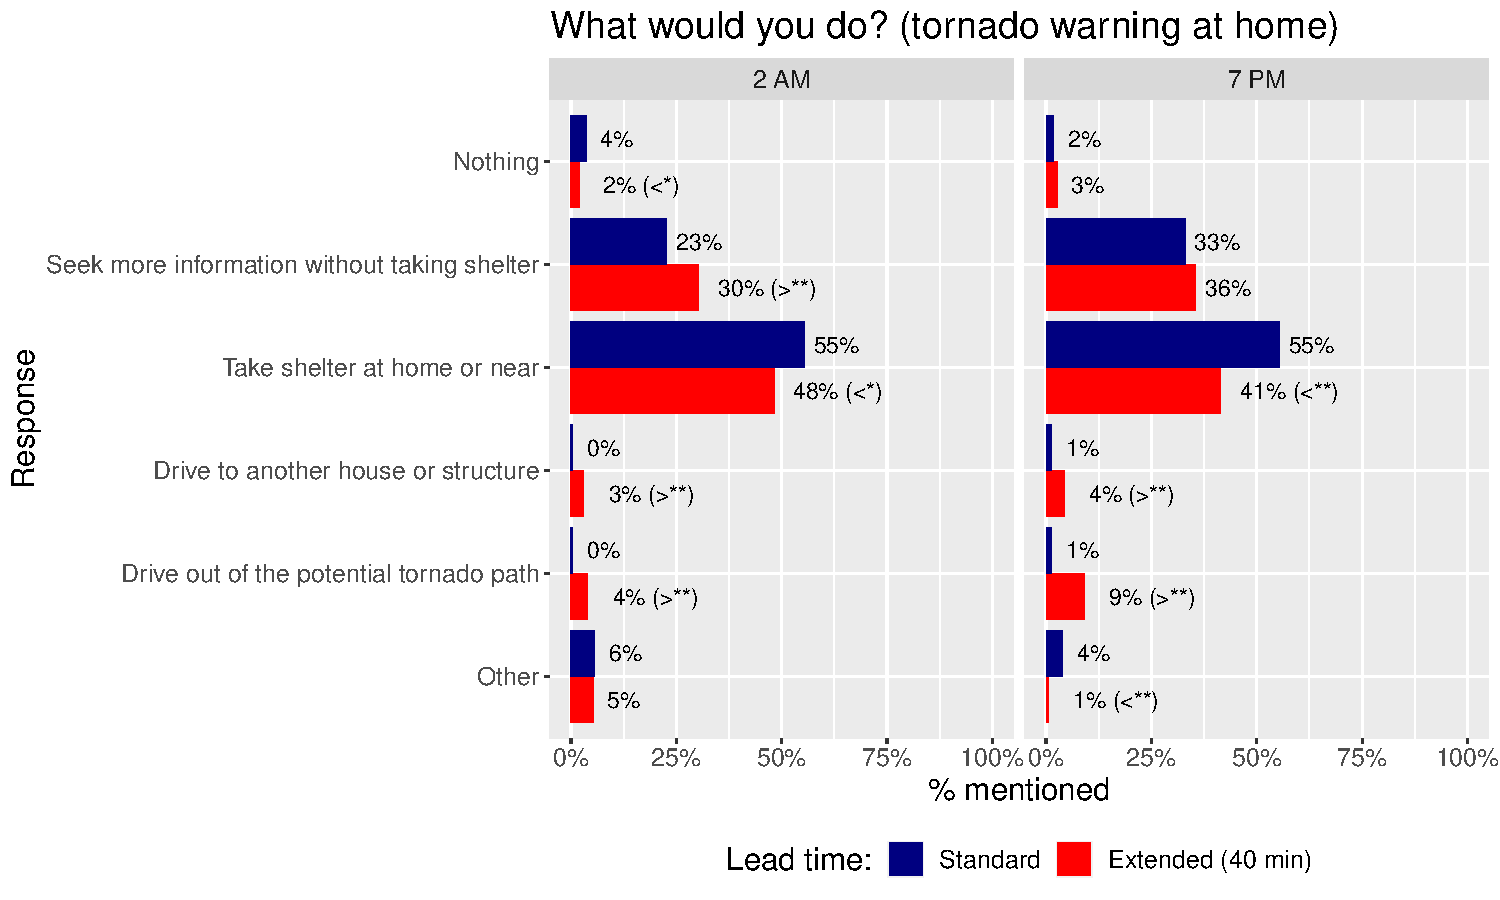
\includegraphics[scale=0.55]{../Graphs/comp_responses_w.pdf} 
\caption{Protective Response by Lead Time (Mail Sample)}\label{comp_responses}
\end{figure}

\begin{figure}[!htbp]
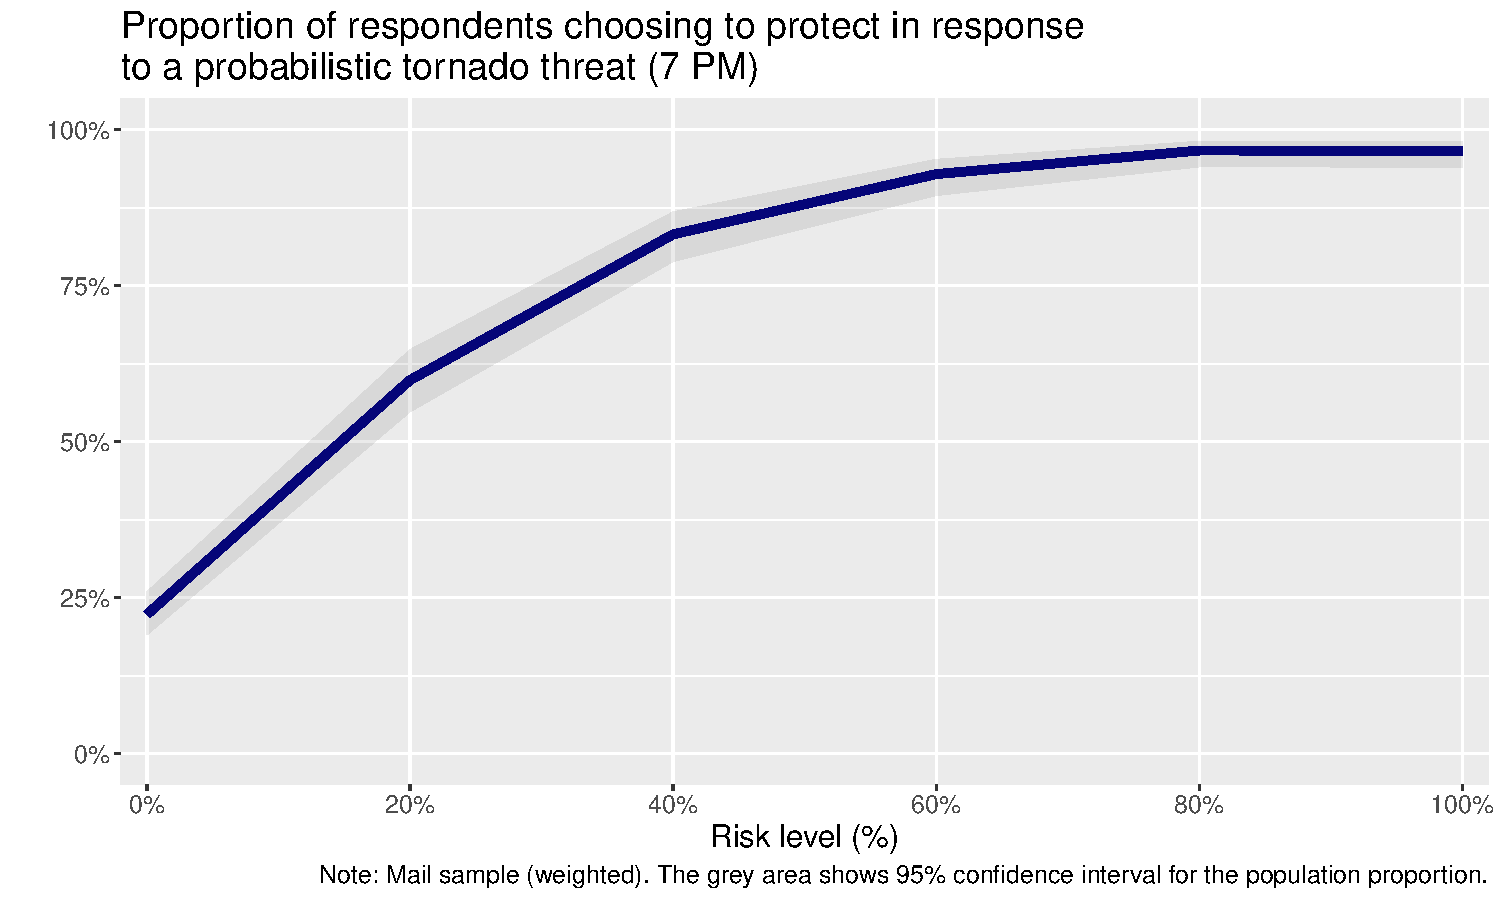
\includegraphics[scale=0.55]{../Graphs/threat_resp_mail_w.pdf} 
\caption{Protective Response by Probability of a Tornado (Mail samples)}\label{threat_resp_mail}
\end{figure}

\newpage
\bibliographystyle{ametsocV6}
\bibliography{references}


\end{document}
%%%%%%%%%%%%%%%%%%%%%%%%%%%%%%%%%%%%%%%%%%%%%%%%%%%%%%%%%%%%%%%%%%%%%
% END OF AMSPAPERV6.1.TEX
%%%%%%%%%%%%%%%%%%%%%%%%%%%%%%%%%%%%%%%%%%%%%%%%%%%%%%%%%%%%%%%%%%%%%